\chapter{Cenni teorici}

In questo capitolo, verrà fornita un'introduzione approfondita agli standard e alle tecnologie che sono stati considerati nell'ambito della nostra attività. La comprensione di tali standard è fondamentale per contestualizzare le scelte progettuali e le strategie implementate. Ci concentreremo su diversi protocolli e specifiche tecniche che hanno influenzato lo sviluppo delle soluzioni adottate, esplorando le loro caratteristiche distintive, le modalità di funzionamento e le applicazioni pratiche.

In particolare, analizzeremo gli standard relativi alla comunicazione wireless nell'ambito \textit{automotive}, come WAVE (\textit{Wireless Access in Vehicular Environments}), che gioca un ruolo cruciale nella connettività dei veicoli e nella gestione delle reti di trasporto intelligenti. 

Successivamente, esamineremo il meccanismo EDCA (\textit{Enhanced Distributed Channel Access}), che è una parte integrante del livello MAC (\textit{Media Access Control}) nel contesto delle reti wireless. EDCA introduce un metodo di accesso al canale più sofisticato rispetto al tradizionale DCF (\textit{Distributed Coordination Function}), permettendo una gestione più efficiente delle priorità di traffico. Questo è particolarmente importante in scenari in cui coesistono diversi tipi di traffico, come video, voce e dati, ognuno con requisiti di latenza e larghezza di banda diversi. Discuteremo come EDCA assegna diverse code di accesso per garantire che le comunicazioni più critiche ricevano la priorità necessaria, migliorando così l'esperienza complessiva degli utenti.

Attraverso questa analisi di WAVE e EDCA, il capitolo intende fornire una comprensione approfondita delle tecnologie che supportano le comunicazioni nei veicoli connessi, evidenziando come queste innovazioni possano contribuire a una mobilità più sicura ed efficiente.

%\section{ITS - Intelligent Transport System}

%\section{VANET}

\section{IEEE WAVE}
WAVE è progettato specificamente per ambienti di trasporto, consentendo la comunicazione tra veicoli (\textit{V2V: Vehicle-to-Vehicle}) e tra veicoli e infrastrutture stradali (\textit{V2I: Vehicle-to-Infrastructure}). Questo protocollo sfrutta canali wireless dedicati per garantire una bassa latenza e una maggiore affidabilità, elementi essenziali per applicazioni critiche come la prevenzione degli incidenti e la gestione del traffico. 

Per facilitare questo, l'IEEE ha introdotto un emendamento specifico al protocollo 802.11, noto come 802.11p\cite{std2007wireless}. Questo emendamento si occupa sia del livello fisico, chiamato PHY, sia della gestione dell'accesso al canale, che riguarda il livello MAC. Non ci soffermeremo ulteriormente sui livelli superiori, se non attraverso un breve excursus, poiché il protocollo in questione supporta senza difficoltà qualsiasi tipo di livello, sia esso basato su IP o meno\cite{DSRC-Based-vehicular}. Degno di nota è il fatto che è stato previsto un apposito protocollo per l'invio di frame che non richiedono un livello di trasporto come TCP o UDP, denominato \textit{WAVE Short Message Protocol (WSMP)}.

\begin{figure}[h!]
    \centering
    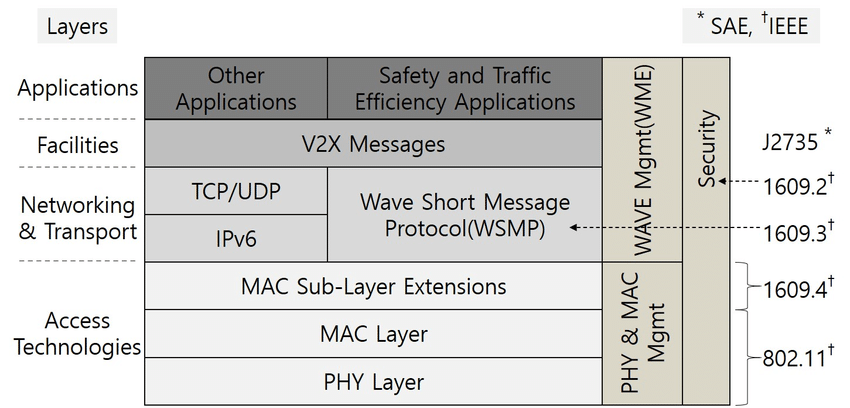
\includegraphics[width=0.7\textwidth]{WAVE-protocol-stack.png}
    \caption{Stack protocollo WAVE}
    \label{fig:wave_stack}
\end{figure}

Di seguito, presentiamo un elenco che fornisce ulteriori dettagli sui protocolli menzionati nella Figura \ref{fig:wave_stack}, partendo dal layer fisico e salendo di volta in volta:

\begin{itemize}
    \item \textit{IEEE 802.11-2016, IEEE Std 802.11p: Wireless Access in Vehicular Environments}.
    \item \textit{IEEE 1609.0: IEEE Guide for Wireless Access in Vehicular Environments (WAVE) Architecture}, con le sue varie componenti\cite{8686445}: 
        \begin{itemize}
            \item \textit{IEEE 1609.4: IEEE Standard for Wireless Access in Vehicular Environments (WAVE) - Multi-Channel Operation}; per il \textit{channel routing} e il \textit{channel coordination}\cite{7435228}.
            \item \textit{IEEE 1609.3: IEEE Standard for Wireless Access in Vehicular Environments (WAVE) - Networking Services}; per i sopracitati \textit{WAVE Short Messages}\cite{9374154}.
            \item \textit{IEEE 1609.2: IEEE Standard for Wireless Access in Vehicular Environments - Security Services for Applications and Management Messages}; per tutti gli aspetti relativi alla sicurezza\cite{10075082}.
        \end{itemize}
\end{itemize}

Risultano, anche, essere presenti altre varie componenti del protocollo \textit{IEEE 1609.0} su cui non ci si soffermerà e si riportano per completezza:

\begin{itemize}
    \item \textit{IEEE 1609.11:  IEEE Standard for Wireless Access in Vehicular Environments (WAVE) - Over-the-Air Electronic Payment Data}; standard per i pagamenti elettronici in applicazione \textit{WAVE based}\cite{5692959}.
    \item \textit{IEEE 1609.12:  IEEE Standard for Wireless Access in Vehicular Environments (WAVE) - Identifier Allocations}; standard per l'allocazione degli identificatori \textit{WAVE}\cite{8877516}.
\end{itemize}

Per concludere, alla luce del fatto che il contesto preso in esame, quello veicolare, richiede uno scambio di informazioni con latenze minime, \textit{WAVE} si basa interamente su una nuova modalità Wireless, simile alla classica \textit{ad hoc}, chiamata \textit{OCB (Outside Context of a Basic Service Set)}. Questo è un approccio che consente la trasmissione di dati al di fuori delle limitazioni tradizionali delle reti Wi-Fi, permettendo una comunicazione più flessibile e diretta tra i dispositivi, senza la necessità di passare attraverso infrastrutture quali i punti di accesso (\textit{Access Point}).

\subsection[Layer fisico]{Layer fisico}
L'IEEE 802.11p è uno standard della famiglia IEEE 802.11 progettato specificamente per la comunicazione wireless in ambienti vehicolari. È una tecnologia di rete che consente la comunicazione tra veicoli e tra veicoli e infrastrutture, facilitando applicazioni come la sicurezza stradale, la gestione del traffico e i servizi di infotainment.

Esso, innanzitutto, è basato su una modulazione OFDM (\textit{Orthogonal Frequencies Division Multiplexing}), ove in un totale di 64 sottoportanti, 48 vengono utilizzate per la trasmissione delle informazioni e 4 sono pilota; supporta velocità differenti in base alla modulazione delle sottoportanti e alla larghezza di banda utilizzati.

Di seguito una tabella riassuntiva dei parametri appena citati, suddivisi per \textit{bandwidth}:

\clearpage % Forza la stampa delle tabelle e figure in sospeso

\begin{table}[htbp]
    \centering
    \begin{tabular}{|p{7em}|p{7em}|p{7em}|p{7em}|} 
     \hline
     \textbf{Parametri} & \textbf{20 MHz} & \textbf{10 MHz} & \textbf{5 MHz} \\ 
     \hline
     \textbf{Bit rate (Mbit/s)} & 6, 9, 12, 18, 24, 36, 48, 54 & 3, 4.5, 6, 9, 12, 18, 24, 27 & 1.5, 2.25, 3, 4.5, 6, 9, 12, 13.5 \\ 
     \hline
     \textbf{Modulation} & BPSK, QPSK, 16/64QAM & BPSK, QPSK, 16/64QAM & BPSK, QPSK, 16/64QAM \\
     \hline
     \textbf{Code rate} & 1/2, 2/3, 3/4 & 1/2, 2/3, 3/4 & 1/2, 2/3, 3/4 \\
     \hline
     \textbf{Subcarriers} & 52 & 52 & 52 \\
     \hline
     \textbf{Spacing} & 312.5 kHz & 156.25 kHz & 78.125 kHz \\ 
     \hline
    \end{tabular}
    \caption{Parametri delle diverse larghezze di banda}
    \label{table:1}
\end{table}

Parlando circa le frequenze utilizzate, l'IEEE 802.11p opera nella banda di frequenza di 5,9 GHz (5,850 - 5,925 GHz), con le larghezze di canale citate nella Tabella \ref{table:1}. Questo standard consente l'uso di circa 9 canali, come illustrato nella Figura \ref{fig:frequency}. Tra questi, i canali 172 (5.860 GHz) e 184 (5.920 GHz) sono dedicati alla sicurezza: il primo fornisce una soluzione robusta per la sicurezza, mentre il secondo funge da protezione contro la congestione su altri canali\cite{ad_hoc_new}.

\begin{figure}[h!]
    \centering
    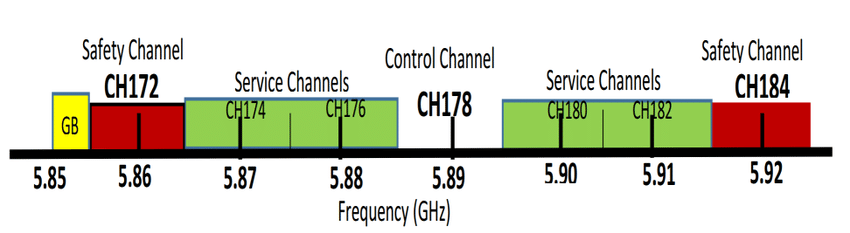
\includegraphics[width=0.7\textwidth]{frequency.png}
    \caption{Frequenze dell'IEEE 802.11p}
    \label{fig:frequency}
\end{figure}

Il canale 178 (5.890 GHz) è un canale di controllo, responsabile della gestione della trasmissione e della creazione del collegamento. Inoltre, sono disponibili sei canali di servizio per la comunicazione bidirezionale tra diversi tipi di unità.

\subsection[Layer MAC]{Layer MAC}
Non esiste una netta distinzione tra il layer MAC dell'IEEE 802.11p con il relativo omonimo del classico IEEE 802.11, se non per alcuni concetti:

\begin{itemize}
    \item come già esplicitato quando si è iniziato a parlare di \textit{WAVE} poc'anzi, esso si basa principalmente sulla modalità \textit{OCB} anzichè le classiche, come ad esempio la \textit{Infrastructure mode}.
    \item per l'accesso al canale, sfrutta una variante della \textit{DCF (Distributed Coordination Function)} chiamata \textit{EDCA (Enhanced Distributed Channel Access)}, sviluppata appositamente per supportare politiche di QoS. A breve verrà affrontato questa nuova \textit{feature} maggiormente nel dettaglio.
\end{itemize}

\subsection[EDCA]{EDCA}
Nell'EDCA, la differenziazione del servizio è garantita attraverso l'assegnazione di diversi parametri di contesa a ciascuna \textit{Access Category (AC)}. Una stazione QoS può supportare fino a otto priorità utente, che vengono mappate su quattro AC. Ogni AC compete per l'accesso al canale utilizzando impostazioni diverse di AIFS (\textit{Arbitration Inter-frame Space}) e CW (\textit{Contention Window})\cite{4024121}; per completezza, si riporta che l'AIFS determina quanto tempo ogni stazione deve attendere prima di poter iniziare a trasmettere, mentre la CW quanto tempo ciascuna stazione deve aspettare in modo casuale prima di tentare di trasmettere.

A differenza della DCF, dove il DIFS (\textit{Distributed Inter-frame Space}) è utilizzato come IFS (\textit{Inter Frame Space}) comune per consentire a una stazione di accedere al canale, l'EDCF (\textit{Enhanced Distributed Channel Function}) adotta AIFS distinti per ciascuna AC al fine di ottenere una differenziazione nell'accesso. L'AIFS per una specifica AC è definito come segue:

\[AIFS[AC] = AIFSN[AC] * \sigma + SIFS\]

\noindent dove
\begin{itemize}
    \item \textit{AIFSN[AC]} denota un numero per differenziare le AIFS per ogni AC diversa (vedi Tabella \ref{table:2});
    \item \textit{\textsigma} \textit{(slot time)} è un intervallo di tempo dipendente dal layer fisico;
    \item \textit{SIFS (\textit{Short Inter Frame Space})} è il tempo tra un frame di dati e uno di ACK.
\end{itemize}

Questi parametri variano in base a determinate caratteristiche della connessione, come la modulazione utilizzata e l'adozione di tecniche MIMO (Tabella \ref{table:2}).
\begin{table}[h!]
    \centering
    \begin{tabular}{|>{\centering\arraybackslash}p{10em}|>{\centering\arraybackslash}p{7em}|>{\centering\arraybackslash}p{7em}|>{\centering\arraybackslash}p{7em}|} 
     \hline
     \textbf{AC} & \textbf{CWmin} & \textbf{CWmax} & \textbf{AIFSN} \\ 
     \hline
     \textbf{AC\_VO (Voice)} & (aCWmin+1)/4-1 & (aCWmin+1)/2-1 & 2 \\ 
     \hline
     \textbf{AC\_VI (Video)} & (aCWmin+1)/2-1 & aCWmin & 2 \\
     \hline
     \textbf{AC\_BE (Best Effort)} & aCWmin & aCWmax & 7 \\
     \hline
     \textbf{AC\_BK (Background)} & aCWmin & aCWmax & 7 \\
     \hline
    \end{tabular}
    \caption{Parametri delle diverse AC}
    \label{table:2}
\end{table}

Nella Tabella \ref{table:3}, invece, sono riportati i parametri nel caso di aCWmin=31 e aCWmax=1023, come usati, per esempio, nel caso di utilizzo di OFDM e MIMO (\textit{IEEE 802.11n}).
\begin{table}[h!]
    \centering
    \begin{tabular}{|>{\centering\arraybackslash}p{10em}|>{\centering\arraybackslash}p{7em}|>{\centering\arraybackslash}p{7em}|>{\centering\arraybackslash}p{7em}|} 
     \hline
     \textbf{AC} & \textbf{CWmin} & \textbf{CWmax} & \textbf{AIFSN} \\ 
     \hline
     \textbf{AC\_VO (Voice)} & 7 & 15 & 2 \\ 
     \hline
     \textbf{AC\_VI (Video)} & 15 & 31 & 2 \\
     \hline
     \textbf{AC\_BE (Best Effort)} & 31 & 1023 & 7 \\
     \hline
     \textbf{AC\_BK (Background)} & 31 & 1023 & 7 \\
     \hline
    \end{tabular}
    \caption{Parametri delle diverse AC}
    \label{table:3}
\end{table}

E' banale notare che la categoria ad accesso prioritario sarà \textit{AC\_V0}, con la priorità che andrà a scendere siano a \textit{AC\_BK}.

Per comprendere la differenziazione del servizio introdotta da AIFS e CW, possiamo considerare l'esempio mostrato nella Figura \ref{fig:aifs}, in cui sono presenti due stazioni, ciascuna con pacchetti in AC1 e AC4. La differenza di AIFSN (AIFS Number) è di 5, il che significa che l'AC1 della STA1 (Stazione 1) ridurrà il suo contatore di backoff 5 slot prima dell'AC4 della STA2 (Stazione 2). Inoltre, durante questo intervallo, il contatore di backoff dell'AC ad alta priorità può arrivare a zero, consentendo la trasmissione del pacchetto. Questo porta all'occupazione del canale a causa della trasmissione del pacchetto ad alta priorità e alla successiva risincronizzazione.

\begin{figure}[h!]
    \centering
    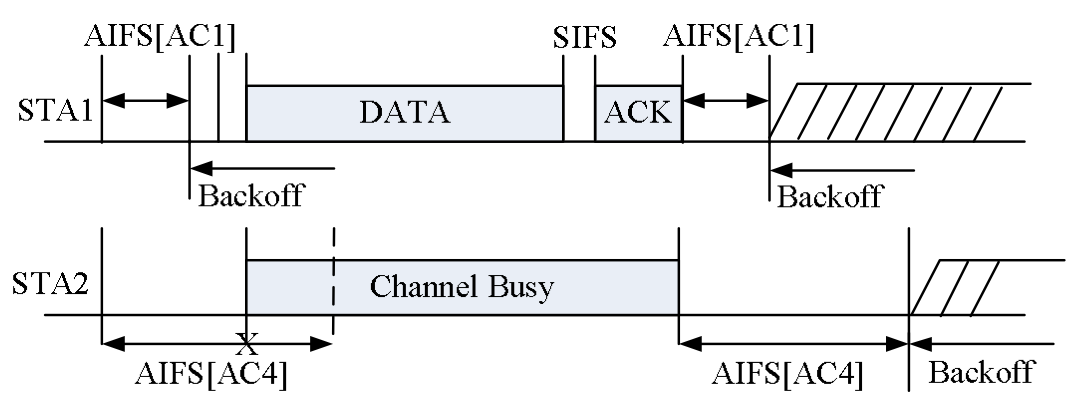
\includegraphics[width=0.7\textwidth]{aifs.png}
    \caption{Accesso al canale nell'EDCA}
    \label{fig:aifs}
\end{figure}

Ad ogni differente AC viene assegnata una differente coda; i vari frame vengono accodati nella coda appropriata in base alla \textit{Class Of Service (CoS)} di appartenenza; quest'ultime risultano essere quelle definite in un altro standard, ovvero l'IEEE 802.1D\cite{1309630}. Il mapping tra classe del frame e AC viene effettuata in questo modo (Tabella \ref{table:4}):

\begin{table}[h!]
    \centering
    \begin{tabular}{|>{\centering\arraybackslash}p{10em}|>{\centering\arraybackslash}p{7em}|} 
     \hline
     \textbf{AC} & \textbf{User Priorities} \\ 
     \hline
     \textbf{AC\_VO (Voice)} & 6, 7 \\ 
     \hline
     \textbf{AC\_VI (Video)} & 4, 5 \\
     \hline
     \textbf{AC\_BE (Best Effort)} & 0, 3 \\
     \hline
     \textbf{AC\_BK (Background)} & 1, 2 \\
     \hline
    \end{tabular}
    \caption{Mappature delle AC con le \textit{User Priorities}}
    \label{table:4}
\end{table}

E', comunque, sempre presente una sorta di casualità tra un AIFSN e un altro in modo da evitare che frame messi nella coda con priorità maggiore monopolizzino il canale a discapito di quelli a priorità minore.

\subsection[IEEE 1609.4 for multi-channel operations]{IEEE 1609.4 for multi-channel operations}